%o handout e o beamer normal serao controlados pelo arquivo normal.tex

%\documentclass[12pt,compess,handout,aspectratio=169]{beamer}
%\usepackage{pgfpages}
%\pgfpagesuselayout{4 on 1}[a4paper,landscape,border shrink=5mm]

%\documentclass[12pt,aspectratio=169]{beamer}
\documentclass[11pt,aspectratio=43]{beamer}
%Para aulas presenciais eu mudei de 11 para 12pt 

%
\usetheme{Boadilla}
\usepackage[utf8]{inputenc}
\usepackage[brazil]{babel}
\usepackage[T1]{fontenc}
\usepackage{mathtools}
%\usepackage{amsmath} mathtools já importa o amsmath
\usepackage{amsfonts}
\usepackage{amssymb}
\usepackage{amsthm}
\usepackage{verbatim}
\usepackage{epsfig}
\usepackage{color}

%para incluir códigos
\usepackage{listings}

\usepackage{multirow}

%esse pacote permite mudar as margens de um unico slide com \begin{adjustwidth}{-1.5em}{-1.5em} e \end{adjustwidth}
\usepackage{changepage}

%Para aulas presenciais eu mudei a margem esquerda dos itemize, assim cabe mais coisa mesmo com a letra maior
\setlength{\leftmargini}{5pt}


%\usepackage[portugues,ruled,linesnumbered,noend]{algorithm2e}
\author{Vinicius de Novaes}
\usepackage{ragged2e}
%pacote para fazer um strikeout na diagonal, cancelar o termo em uma equação.
\usepackage{cancel}

\usepackage{tikz, tkz-graph, pgfplots}
\usepackage{tikz-qtree}

\usetikzlibrary{arrows,positioning,chains,fit,shapes,calc,backgrounds,quotes,patterns}
\usetikzlibrary{snakes,arrows.meta}
\usetikzlibrary{positioning}
\usetikzlibrary{decorations.markings}

\usepgfplotslibrary{fillbetween}

\newcommand\pgfmathsinandcos[3]{% 
  \pgfmathsetmacro#1{sin(#3)}% 
  \pgfmathsetmacro#2{cos(#3)}% 
}



\usepackage{epsdice}


%pacote para fazer uma bela caixa
\usepackage[framemethod=tikz]{mdframed}
\definecolor{myblue}{rgb}{0.122, 0.435, 0.698}

\newmdenv[innerlinewidth=0.5pt, roundcorner=4pt,linecolor=myblue,innerleftmargin=6pt,
innerrightmargin=6pt,innertopmargin=6pt,innerbottommargin=6pt]{mybox}


%Meus blocks personalizados
\newenvironment{definição}{%
  \setbeamercolor{block body}{bg=green!10,fg=black}
  \setbeamercolor{block title}{bg=green!30,fg=black}
  \begin{block}{Definição}}{\end{block}}

%minhas cores (pacote colors)
\definecolor{mygreen}{rgb}{0,0.6,0}
\definecolor{mygray}{rgb}{0.5,0.5,0.5}
\definecolor{mymauve}{rgb}{0.58,0,0.82}

%Configuração do listings
\lstset{ %
  backgroundcolor=\color{white},   % choose the background color; you must add \usepackage{color} or \usepackage{xcolor}
%  basicstyle=\footnotesize,        % the size of the fonts that are used for the code
%  breakatwhitespace=false,         % sets if automatic breaks should only happen at whitespace
%  breaklines=true,                 % sets automatic line breaking
%  captionpos=b,                    % sets the caption-position to bottom
  commentstyle=\color{mygreen},    % comment style
%  deletekeywords={...},            % if you want to delete keywords from the given language
  escapeinside=||,          % if you want to add LaTeX within your code
%  extendedchars=true,              % lets you use non-ASCII characters; for 8-bits encodings only, does not work with UTF-8
%  frame=single,	                   % adds a frame around the code
%  keepspaces=true,                 % keeps spaces in text, useful for keeping indentation of code (possibly needs columns=flexible)
  keywordstyle=\color{blue},       % keyword style
%  language=Octave,                 % the language of the code
%  otherkeywords={*,...},           % if you want to add more keywords to the set
%  numbers=left,                    % where to put the line-numbers; possible values are (none, left, right)
 % numbersep=5pt,                   % how far the line-numbers are from the code
%  numberstyle=\tiny\color{mygray}, % the style that is used for the line-numbers
%  rulecolor=\color{black},         % if not set, the frame-color may be changed on line-breaks within not-black text (e.g. comments (green here))
%  showspaces=false,                % show spaces everywhere adding particular underscores; it overrides 'showstringspaces'
  showstringspaces=false,          % underline spaces within strings only
%  showtabs=false,                  % show tabs within strings adding particular underscores
%  stepnumber=2,                    % the step between two line-numbers. If it's 1, each line will be numbered
%  stringstyle=\color{mymauve},     % string literal style
%  tabsize=2,	                   % sets default tabsize to 2 spaces
%  title=\lstname                   % show the filename of files included with \lstinputlisting; also try caption instead of title
}


\title{Algoritmos}
%\setbeamercovered{transparent} 


%Esse snipet aqui é para tentar fazer o \pause funcionar dentro do align
\makeatletter
\let\save@measuring@true\measuring@true
\def\measuring@true{%
  \save@measuring@true
  \def\beamer@sortzero##1{\beamer@ifnextcharospec{\beamer@sortzeroread{##1}}{}}%
  \def\beamer@sortzeroread##1<##2>{}%
  \def\beamer@finalnospec{}%
}
\makeatother

%\logo{} 
%\institute{} 
\date{} 
%\subject{} 

\beamertemplatenavigationsymbolsempty
\setbeamertemplate{footline}[frame number]

%\setbeamertemplate{navigation symbols}{%
%    \usebeamerfont{footline}%
%    \usebeamercolor[fg]{footline}%
%    \hspace{1em}%
%    \insertframenumber/\inserttotalframenumber
%}
%\setbeamercolor{footline}{fg=black}
%\setbeamerfont{footline}{series=\bfseries}
\setbeamersize{text margin left=10mm,text margin right=10mm} 

\mode<beamer|second|trans|article>{\newcommand{\onlyhandout}[1]{}}
\mode<handout|second|trans|article>{\newcommand{\onlybeamer}[1]{}}
\mode<handout>{\newcommand{\onlyhandout}[1]{#1}}
\mode<beamer>{\newcommand{\onlybeamer}[1]{#1}}

\newcommand{\spitem}[1]{\begin{itemize}
\pitem #1
\end{itemize}} 
\newcommand{\pitem}{\pause\item}  
\newcommand{\ppause}{\pause}  
%antes de descomentar esse aqui, tente descomentar a primeira linha desse arquivo
%\newcommand{\pitem}{\item}  
%\newcommand{\ppause}{} 

\patchcmd{\theorem}{Theorem}{Teorema}{}{}
\patchcmd{\lemma}{Lemma}{Lema}{}{}
\patchcmd{\theorem}{defi}{Definição}{}{}

%FORMATAÇÃO, CORES 
\newcommand{\azul}[1]{{\color{blue}{#1}}}
\newcommand{\verm}[1]{{\color{red}{#1}}}
\definecolor{myGreen}{rgb}{0,0.7,0}
\newcommand{\verde}[1]{{\color{myGreen}{#1}}}
\newcommand{\roxo}[1]{{\color{magenta}{#1}}}


\include{macros}
\begin{document}

\begin{frame}
\titlepage
\end{frame}

%\begin{frame}{}
%\begin{itemize}
%\item Semanalmente um questionário individual valendo nota e presença. 
%\item Publicado na sexta com entrega até terça antes da aula.
%\item Seja $Q_t$ sua nota nos questionários do bimestre $t$ de 0 a 1.
%\item Nota $P_t$ dos trabalhos práticos do bimestre $t$ de 0 a 10.
%\item Nota do bimestre $t$, $N_t = P_t \times Q_t$.
%\item Nota final $M = \frac{N_1 + N_2}{2}$
%\item Se frequência menor que $75\%$ o aluno reprovou-se.
%\item Senão se, $M \geq 6$ e presença maior que $75\%$ o aluno aprovou-se.
%\item Senão se, $M < 6$ e presença maior que $75\%$ o aluno pode fazer uma substitutiva que substitui a menor entre $N_1$ e $N_2$.
%\end{itemize}
%\end{frame}
%



% \begin{frame}{Fontes}
% \tiny
% \begin{itemize}
% \item $[clrs]$ Algoritmos: Teoria e Prática (Terceira Edição) Thomas H. Cormen, Charles Eric Leiserson, Ronald Rivest e Clifford Stein. 

% \item $[timr]$ Algorithms Illuminated Series, Tim Roughgarden 

% \item Desmistificando Algoritmos, Thomas H. Cormen.

% \item Algoritmos, Sanjoy Dasgupta, Christos Papadimitriou e Umesh Vazirani 

% \item Stanford Algorithms

% \url{https://www.youtube.com/playlist?list=PLXFMmlk03Dt7Q0xr1PIAriY5623cKiH7V}

% \url{https://www.youtube.com/playlist?list=PLXFMmlk03Dt5EMI2s2WQBsLsZl7A5HEK6}

% \item Conjunto de Slides dos Professores Cid C. de Souza, Cândida N. da Silva, Orlando Lee, Pedro J. de Rezende

% \item Conjunto de Slides do Professores Cid C. de Souza para a disciplina MO420
% \end{itemize}
% Qualquer erro é de minha responsabilidade.
% \end{frame}



%\input{aula01}
%\input{aula01_revisao}
%\input{aula02}
%\input{aula02_revisao}
%\input{aula03}
%\input{aula03_revisao}
%\input{aula04} 
%\input{aula04_revisao}
%\input{aula05}
%\input{aula05_revisao}
%\input{aula06}
%\input{aula04} 
%\input{aula04_revisao}
%\input{aula07}
%\input{aula07_revisao}
%\input{aula08}
%\input{probabilidade_revisao} %Tem dentro da aula 9
%\input{aula09}
%\input{aula09_revisao}
%\input{aula10}
%\input{aula10_revisao}
%\input{aula11}
%\input{aula11_revisao}
%\input{probabilidade_condicional_revisao}
%\input{aula12}
%\input{aula12_revisao}
%\input{aula13}
%\input{aula13_revisao}
%\input{aula14}
%\input{aula14_revisao}
%\input{aula15}
%\input{caminho_minimo_nao_ponderado_BFS_revisao}
%\input{aula16}
%\input{aula17} %Já inclui uma revisão sobre Dijkstra
%\input{aula17_revisao}
%\input{aula18}
%\input{aula19}
%\input{aula20}
%\input{mod21-01-PD} desnecessário, tudo aqui já tá no KNAP
%\input{mod21-02-Knap}
%\input{mod21-03-BF} % Contém uma Revisão do Dijkstra
%\input{mod21-BF-revisao}
%\input{mod21-04-FW}
%\input{mod21-FW-revisao}
%\input{mod21-05-Johnson}
%\input{mod22-01-Poli} %versão mais superficial
%\input{mod22-02-NP-NPC}%versão mais profunda, tem coisas repetidas da anterior
%\input{mod22-02-NP-NPC-revisao}
%\input{mod22-03-3-cnf}
%\input{mod23-04-sat}
%\input{mod23-05-hamCicle}
%\input{mod23-tsp-subsetsum}
%\begin{frame}
%\centering
%\includegraphics[scale=0.5]{figs/arvore_provas_np.png}
%\end{frame}
%\input{mod23-solving_vertex_cover}
%\input{mod24-knap}
%\input{mod25-localSearch} %Nao tá feito
\begin{frame}{Fundamentos de Criptografia}{}
\begin{itemize}
\pitem Quando fazemos compras pela internet, temos que enviar o número do cartão de crédito para efetivar a compra.
\item A internet é uma rede pública, e qualquer um pode acessar os pacotes de dados que são transmitidos através dela.
\pitem É mais seguro se você disfarçar os dados do seu cartão de alguma maneira.
\item E é o que fazemos quando, por exemplo, usamos um site que começa com ``https'' ao invés de ``http''.
\end{itemize}
\end{frame}


\begin{frame}{}{}
\begin{itemize}
\pitem Muitas informações podem ser roubadas em conexões pela internet.
\item Informações enviadas de/para forças armadas, diplomáticas,  cartão de crédito, etc...
\pitem Portanto além de precisarmos de formas de criptografar e decifrar informações, esse métodos precisam ser dificílimos de derrotar.
\end{itemize}
\end{frame}



\begin{frame}{}{}
\begin{tikzpicture}[shorten >=1pt,scale=0.6]%,on grid
\footnotesize
\tikzstyle{fantasma}=[minimum size=0cm]
\tikzstyle{bolota}=[shape=circle,thick,draw,minimum size=1.5cm]


\node[fantasma] at (0,0) (Alice) {Alice};
\node[shape=rectangle,thick,draw] at (6,0) (encr) {$f(M)$};
\node[shape=rectangle,thick,draw] at (12,0) (dese) {$g(C)$};
\node[fantasma] at (18,0) (Bob) {Bob};


\path[->,draw,thick] (Alice) edge node[fill=white, anchor=north, pos=0.5, align=center,yshift=-5pt] {$M$\\ Texto comum\\ (plain text)} (encr);

\path[->,draw,thick] (encr) edge node[fill=white, anchor=north, pos=0.5, align=center,yshift=-5pt] {$C$\\ Texto cifrado\\ (ciphertext)} (dese);

\path[->,draw,thick] (dese) edge node[fill=white, anchor=north, pos=0.5, align=center,yshift=-5pt] {$M$} (Bob);


\visible<2->{\node[fantasma] at (9,4) (Mau) {Maurício};}
\node<2->[fantasma] at (9,0) (C) {};
\path<2->[->,draw,thick] (C) -- (Mau);

\node<3->[fantasma] at (6,1) (chave1) {$chave$};
\node<3->[fantasma] at (12,1) (chave1) {$chave$};
\end{tikzpicture}
\end{frame}



\begin{frame}{Cifra de deslocamento}{}
\begin{itemize}
\pitem Supostamente, Júlio César teria se comunicado com seus generais usando uma cifra de deslocamento.
\pitem Nessa cifra substitui-se cada letra pela que aparece 3 lugares adiante no alfabeto. \ppause

\begin{center}
\begin{tikzpicture}[shorten >=1pt,scale=0.7]%,on grid
\footnotesize
\tikzstyle{fantasma}=[minimum size=0cm]
\tikzstyle{bolota}=[shape=circle,thick,draw,minimum size=1.5cm]


\node[fantasma] at (0,0) (A) {A};
\node[fantasma] at (1,0) (B) {B};
\node[fantasma] at (2,0) (C) {C};
\node[fantasma] at (3,0) (D) {D};
\node[fantasma] at (4,0) (E) {E};
\node[fantasma] at (5,0) (F) {F};
\node[fantasma] at (6,0) (etc) {\ldots};


\draw[->,thick] (A.north) to [bend left=45] (D.north);
\draw[->,thick] (B.north) to [bend left=45] (E.north);
\draw[->,thick] (C.north) to [bend left=45] (F.north);
\draw[->,thick] (D.north) to [bend left=45] (etc.north);
\end{tikzpicture}
\end{center}
\pitem Nesse caso a $chave$ é 3 o que é muito óbvio, então se quisermos usar a cifra de deslocamento, o ideal seria escolher outra chave. 
\end{itemize}
\end{frame}


\begin{frame}{}{}
\begin{center}
inkzxjegtrg\ppause
\end{center}
\begin{columns}[t]\small
\begin{column}{0.33\textwidth}
0: inkzxjegtrg\\\ppause
1: hmjywidfsqf\\
2: glixvhcerpe\\
3: fkhwugbdqod\\
4: ejgvtfacpnc\\
\only<3>{5: difuse bomb\\}
\only<4->{\bf \small 5: difuse bomb\\}
\end{column}
\begin{column}{0.33\textwidth}
6: chetrdzanla\\
7: bgdsqcy mk \\
8: afcrpbxzljz\\
9:  ebqoawykiy\\
10: zdapn vxjhx\\
11: yc omzuwigw\\
12: xbznlytvhfv\\
13: waymkxsugeu\\
\end{column}
\begin{column}{0.33\textwidth}
14: v xljwrtfdt\\
15: uzwkivqsecs\\
16: tyvjhuprdbr\\
17: sxuigtoqcaq\\
18: rwthfsnpb p\\
19: qvsgermoazo\\
20: purfdqln yn\\
21: otqecpkmzxm\\
22: nspdbojlywl\\
23: mrocanikxvk\\
24: lqnb mhjwuj\\
25: kpmazlgivti\\
26: jol ykfhush\ppause
\end{column}
\end{columns}
\begin{center}
\ppause
difuse bomb
\end{center}
\end{frame}



\begin{frame}{Cifra de substituição simples}{}
\begin{itemize}
\pitem Na cifra de deslocamento existem 26 chaves distintas, fácil de testar todas.
\pitem Mas podemos fazer algo mais seguro substituindo cada carácter por outro qualquer, não necessariamente o que está a 3 posições no alfabeto.
\end{itemize}
\ppause 

\ \\

{\footnotesize
\begin{tabular}{|p{0.14cm}|p{0.14cm}|p{0.14cm}|p{0.14cm}|p{0.14cm}|p{0.14cm}|p{0.14cm}|p{0.14cm}|p{0.14cm}|p{0.14cm}|p{0.14cm}|p{0.14cm}|p{0.14cm}|p{0.14cm}|p{0.14cm}|p{0.14cm}|p{0.14cm}|p{0.14cm}|p{0.14cm}|p{0.14cm}|p{0.14cm}|p{0.14cm}|p{0.14cm}|p{0.14cm}|p{0.14cm}|p{0.14cm}|}
\hline
a & b & c & d & e & f & g & h & i & j & k & l & m & n & o & p & q & r & s & t & u & v & w & x & y & z \\\hline
\end{tabular}

\begin{tabular}{|p{0.14cm}|p{0.14cm}|p{0.14cm}|p{0.14cm}|p{0.14cm}|p{0.14cm}|p{0.14cm}|p{0.14cm}|p{0.14cm}|p{0.14cm}|p{0.14cm}|p{0.14cm}|p{0.14cm}|p{0.14cm}|p{0.14cm}|p{0.14cm}|p{0.14cm}|p{0.14cm}|p{0.14cm}|p{0.14cm}|p{0.14cm}|p{0.14cm}|p{0.14cm}|p{0.14cm}|p{0.14cm}|p{0.14cm}|}
\hline
u & w & l & x & q & f & p & r & e & n & v & h & z & t & j & s & c & g & i & a & k & o & d & m & y & b \\\hline
\end{tabular}}
\end{frame}



\begin{frame}{}{}
\begin{itemize}
\pitem Agora existem $26!$ permutações (chaves) diferente, difícil de testar uma a uma.
\pitem Entretanto ainda é bastante fácil descobrir um texto criptografado dessa maneira.
\end{itemize}
\end{frame}



\begin{frame}{}{}
\small
\begin{columns}
\begin{column}{0.8\textwidth}
\texttt{j wjzwugxqej gkiij fje j sgezqegj pgutxq uauckq qz veqo xqixq j fetuh xq uwgeh tui khaezui iqzutui u gkiieu ljtlqtagjk iku jfqtieou sgetlesuhzqtaq tui hetrui xq fgqtaq tj hqiaq q tj ikh qzwjgu zjiljk jluiejtuhzqtaq uauckq jkagji hkpugqi tu luzsutru sugu xqiagkeg u etfguqiagkakgu zeheaug xu klguteu q whjckqug gqzqiiui xq ugzui jlexqtauei}
\begin{itemize}
\pitem Uma ideia é usar frequência de cada carácter, se soubermos que o texto está em português.
\end{itemize}
\end{column}
\begin{column}{0.2\textwidth}
\begin{tabular}{l|r}
u	& 41\\
q	& 33\\
i	& 26\\
g	& 24\\
j	& 22\\
e	& 21\\
t	& 21
\end{tabular}

Em pt-br.
\begin{tabular}{l|r}
  a & 	14.63\%\\
  e	& 12.57\%\\
  o	& 10.73\%\\
  s	& 7.81\%\\
  r	& 6.53\%\\
  i	& 6.18\%\\
  n	& 5.05\%
\end{tabular}
\end{column}
\end{columns}
\end{frame}


\begin{frame}{}{}
\small
\begin{columns}
\begin{column}{0.8\textwidth}
\begin{itemize}
\item u deve ser A.
\end{itemize}
\texttt{j wjzwAgxqej gkiij fje j sgezqegj pgAtxq AaAckq qz veqo xqixq j fetAh xq Awgeh tAi khaezAi iqzAtAi A gkiieA ljtlqtagjk ikA jfqtieoA sgetlesAhzqtaq tAi hetrAi xq fgqtaq tj hqiaq q tj ikh qzwjgA zjiljk jlAiejtAhzqtaq AaAckq jkagji hkpAgqi tA lAzsAtrA sAgA xqiagkeg A etfgAqiagkakgA zeheaAg xA klgAteA q whjckqAg gqzqiiAi xq AgzAi jlexqtaAei}
\begin{itemize}
\item Parece ok.
\end{itemize}
\end{column}
\begin{column}{0.2\textwidth}
\begin{tabular}{l|r}
u	& 41\\
q	& 33\\
i	& 26\\
g	& 24\\
j	& 22\\
e	& 21\\
t	& 21
\end{tabular}

Em pt-br.
\begin{tabular}{l|r}
  a & 	14.63\%\\
  e	& 12.57\%\\
  o	& 10.73\%\\
  s	& 7.81\%\\
  r	& 6.53\%\\
  i	& 6.18\%\\
  n	& 5.05\%
\end{tabular}
\end{column}
\end{columns}
\end{frame}


\begin{frame}{}{}
\small
\begin{columns}
\begin{column}{0.8\textwidth}
\begin{itemize}
\item q deve ser E.
\end{itemize}
\texttt{j wjzwAgxEej gkiij fje j sgezEegj pgAtxE AaAckE Ez veEo xEixE j fetAh xE Awgeh tAi khaezAi iEzAtAi A gkiieA ljtlEtagjk ikA jfEtieoA sgetlesAhzEtaE tAi hetrAi xE fgEtaE tj hEiaE E tj ikh EzwjgA zjiljk jlAiejtAhzEtaE AaAckE jkagji hkpAgEi tA lAzsAtrA sAgA xEiagkeg A etfgAEiagkakgA zeheaAg xA klgAteA E whjckEAg gEzEiiAi xE AgzAi jlexEtaAei}
\begin{itemize}
\item Parece ok.
\end{itemize}
\end{column}
\begin{column}{0.2\textwidth}
\begin{tabular}{l|r}
u	& 41\\
q	& 33\\
i	& 26\\
g	& 24\\
j	& 22\\
e	& 21\\
t	& 21
\end{tabular}

Em pt-br.
\begin{tabular}{l|r}
  a & 	14.63\%\\
  e	& 12.57\%\\
  o	& 10.73\%\\
  s	& 7.81\%\\
  r	& 6.53\%\\
  i	& 6.18\%\\
  n	& 5.05\%
\end{tabular}
\end{column}
\end{columns}
\end{frame}

\begin{frame}{}{}
\small
\begin{columns}
\begin{column}{0.8\textwidth}
\begin{itemize}
\item i deve ser O.
\end{itemize}
\texttt{j wjzwAgxEej gkOOj fje j sgezEegj pgAtxE AaAckE Ez veEo xEOxE j fetAh xE Awgeh tAO khaezAO OEzAtAO A gkOOeA ljtlEtagjk OkA jfEtOeoA sgetlesAhzEtaE tAO hetrAO xE fgEtaE tj hEOaE E tj Okh EzwjgA zjOljk jlAOejtAhzEtaE AaAckE jkagjO hkpAgEO tA lAzsAtrA sAgA xEOagkeg A etfgAEOagkakgA zeheaAg xA klgAteA E whjckEAg gEzEOOAO xE AgzAO jlexEtaAeO}
\begin{itemize}
\item Ficou estranho, note o OOAO. Pode ser S
\end{itemize}
\end{column}
\begin{column}{0.2\textwidth}
\begin{tabular}{l|r}
u	& 41\\
q	& 33\\
i	& 26\\
g	& 24\\
j	& 22\\
e	& 21\\
t	& 21
\end{tabular}

Em pt-br.
\begin{tabular}{l|r}
  a & 	14.63\%\\
  e	& 12.57\%\\
  o	& 10.73\%\\
  s	& 7.81\%\\
  r	& 6.53\%\\
  i	& 6.18\%\\
  n	& 5.05\%
\end{tabular}
\end{column}
\end{columns}
\end{frame}


\begin{frame}{}{}
\small
\begin{columns}
\begin{column}{0.8\textwidth}
\begin{itemize}
\item (i)O deve ser S.
\end{itemize}
\texttt{j wjzwAgxEej gkSSj fje j sgezEegj pgAtxE AaAckE Ez veEo xESxE j fetAh xE Awgeh tAS khaezAS SEzAtAS A gkSSeA ljtlEtagjk SkA jfEtSeoA sgetlesAhzEtaE tAS hetrAS xE fgEtaE tj hESaE E tj Skh EzwjgA zjSljk jlASejtAhzEtaE AaAckE jkagjS hkpAgES tA lAzsAtrA sAgA xESagkeg A etfgAESagkakgA zeheaAg xA klgAteA E whjckEAg gEzESSAS xE AgzAS jlexEtaAeS}
\begin{itemize}
\item Parece Ok.
\end{itemize}
\end{column}
\begin{column}{0.2\textwidth}
\begin{tabular}{l|r}
u	& 41\\
q	& 33\\
i	& 26\\
g	& 24\\
j	& 22\\
e	& 21\\
t	& 21
\end{tabular}

Em pt-br.
\begin{tabular}{l|r}
  a & 	14.63\%\\
  e	& 12.57\%\\
  o	& 10.73\%\\
  s	& 7.81\%\\
  r	& 6.53\%\\
  i	& 6.18\%\\
  n	& 5.05\%
\end{tabular}
\end{column}
\end{columns}
\end{frame}


\begin{frame}{}{}
\small
\begin{columns}
\begin{column}{0.8\textwidth}
\begin{itemize}
\item g deve ser O.
\end{itemize}
\texttt{j wjzwAOxEej OkSSj fje j sOezEeOj pOAtxE AaAckE Ez veEo xESxE j fetAh xE AwOeh tAS khaezAS SEzAtAS A OkSSeA ljtlEtaOjk SkA jfEtSeoA sOetlesAhzEtaE tAS hetrAS xE fOEtaE tj hESaE E tj Skh EzwjOA zjSljk jlASejtAhzEtaE AaAckE jkaOjS hkpAOES tA lAzsAtrA sAOA xESaOkeO A etfOAESaOkakOA zeheaAO xA klOAteA E whjckEAO OEzESSAS xE AOzAS jlexEtaAeS}
\begin{itemize}
\item Note a palavra OEzESSAS. Deve ser R
\end{itemize}
\end{column}
\begin{column}{0.2\textwidth}
\begin{tabular}{l|r}
u	& 41\\
q	& 33\\
i	& 26\\
g	& 24\\
j	& 22\\
e	& 21\\
t	& 21
\end{tabular}

Em pt-br.
\begin{tabular}{l|r}
  a & 	14.63\%\\
  e	& 12.57\%\\
  o	& 10.73\%\\
  s	& 7.81\%\\
  r	& 6.53\%\\
  i	& 6.18\%\\
  n	& 5.05\%
\end{tabular}
\end{column}
\end{columns}
\end{frame}



\begin{frame}{}{}
\small
\begin{columns}
\begin{column}{0.8\textwidth}
\begin{itemize}
\item (g)O deve ser R.
\end{itemize}
\texttt{j wjzwARxEej RkSSj fje j sRezEeRj pRAtxE AaAckE Ez veEo xESxE j fetAh xE AwReh tAS khaezAS SEzAtAS A RkSSeA ljtlEtaRjk SkA jfEtSeoA sRetlesAhzEtaE tAS hetrAS xE fREtaE tj hESaE E tj Skh EzwjRA zjSljk jlASejtAhzEtaE AaAckE jkaRjS hkpARES tA lAzsAtrA sARA xESaRkeR A etfRAESaRkakRA zeheaAR xA klRAteA E whjckEAR REzESSAS xE ARzAS jlexEtaAeS}
\begin{itemize}
\item Parece ok.
\end{itemize}
\end{column}
\begin{column}{0.2\textwidth}
\begin{tabular}{l|r}
u	& 41\\
q	& 33\\
i	& 26\\
g	& 24\\
j	& 22\\
e	& 21\\
t	& 21
\end{tabular}

Em pt-br.
\begin{tabular}{l|r}
  a & 	14.63\%\\
  e	& 12.57\%\\
  o	& 10.73\%\\
  s	& 7.81\%\\
  r	& 6.53\%\\
  i	& 6.18\%\\
  n	& 5.05\%
\end{tabular}
\end{column}
\end{columns}
\end{frame}



\begin{frame}{}{}
\small
\begin{columns}
\begin{column}{0.8\textwidth}
\begin{itemize}
\item j deve ser O.
\end{itemize}
\texttt{O wOzwARxEeO RkSSO fOe O sRezEeRO pRAtxE AaAckE Ez veEo xESxE O fetAh xE AwReh tAS khaezAS SEzAtAS A RkSSeA lOtlEtaROk SkA OfEtSeoA sRetlesAhzEtaE tAS hetrAS xE fREtaE tO hESaE E tO Skh EzwORA zOSlOk OlASeOtAhzEtaE AaAckE OkaROS hkpARES tA lAzsAtrA sARA xESaRkeR A etfRAESaRkakRA zeheaAR xA klRAteA E whOckEAR REzESSAS xE ARzAS OlexEtaAeS}
\begin{itemize}
\item Parece ok.
\end{itemize}
\end{column}
\begin{column}{0.2\textwidth}
\begin{tabular}{l|r}
u	& 41\\
q	& 33\\
i	& 26\\
g	& 24\\
j	& 22\\
e	& 21\\
t	& 21
\end{tabular}

Em pt-br.
\begin{tabular}{l|r}
  a & 	14.63\%\\
  e	& 12.57\%\\
  o	& 10.73\%\\
  s	& 7.81\%\\
  r	& 6.53\%\\
  i	& 6.18\%\\
  n	& 5.05\%

\end{tabular}
\end{column}
\end{columns}
\end{frame}


\begin{frame}{}{}
\small
\begin{columns}
\begin{column}{0.8\textwidth}
\begin{itemize}
\item e deve ser I.
\end{itemize}
\texttt{O wOzwARxEIO RkSSO fOI O sRIzEIRO pRAtxE AaAckE Ez vIEo xESxE O fItAh xE AwRIh tAS khaIzAS SEzAtAS A RkSSIA lOtlEtaROk SkA OfEtSIoA sRItlIsAhzEtaE tAS hItrAS xE fREtaE tO hESaE E tO Skh EzwORA zOSlOk OlASIOtAhzEtaE AaAckE OkaROS hkpARES tA lAzsAtrA sARA xESaRkIR A ItfRAESaRkakRA zIhIaAR xA klRAtIA E whOckEAR REzESSAS xE ARzAS OlIxEtaAIS}
\begin{itemize}
\item Parece ok.
\end{itemize}
\end{column}
\begin{column}{0.2\textwidth}
\begin{tabular}{l|r}
u	& 41\\
q	& 33\\
i	& 26\\
g	& 24\\
j	& 22\\
e	& 21\\
t	& 21
\end{tabular}

Em pt-br.
\begin{tabular}{l|r}
  a & 	14.63\%\\
  e	& 12.57\%\\
  o	& 10.73\%\\
  s	& 7.81\%\\
  r	& 6.53\%\\
  i	& 6.18\%\\
  n	& 5.05\%
\end{tabular}
\end{column}
\end{columns}
\end{frame}


\begin{frame}{}{}
\small
\begin{columns}
\begin{column}{0.8\textwidth}
\begin{itemize}
\item t deve ser N.
\end{itemize}
\texttt{O wOzwARxEIO RkSSO fOI O sRIzEIRO pRANxE AaAckE Ez vIEo xESxE O fINAh xE AwRIh NAS khaIzAS SEzANAS A RkSSIA lONlENaROk SkA OfENSIoA sRINlIsAhzENaE NAS hINrAS xE fRENaE NO hESaE E NO Skh EzwORA zOSlOk OlASIONAhzENaE AaAckE OkaROS hkpARES NA lAzsANrA sARA xESaRkIR A INfRAESaRkakRA zIhIaAR xA klRANIA E whOckEAR REzESSAS xE ARzAS OlIxENaAIS}
\begin{itemize}
\item Parece ok.
\end{itemize}
\end{column}
\begin{column}{0.2\textwidth}
\begin{tabular}{l|r}
u	& 41\\
q	& 33\\
i	& 26\\
g	& 24\\
j	& 22\\
e	& 21\\
t	& 21
\end{tabular}

Em pt-br.
\begin{tabular}{l|r}
  a & 	14.63\%\\
  e	& 12.57\%\\
  o	& 10.73\%\\
  s	& 7.81\%\\
  r	& 6.53\%\\
  i	& 6.18\%\\
  n	& 5.05\%
\end{tabular}
\end{column}
\end{columns}
\end{frame}


\begin{frame}{}{}
\small
\begin{itemize}
\item O próximo seria k por D.
\end{itemize}
\texttt{O wOzwARxEIO RDSSO fOI O sRIzEIRO pRANxE AaAcDE Ez vIEo xESxE O fINAh xE AwRIh NAS DhaIzAS SEzANAS A RDSSIA lONlENaROD SDA OfENSIoA sRINlIsAhzENaE NAS hINrAS xE fRENaE NO hESaE E NO SDh EzwORA zOSlOD OlASIONAhzENaE AaAcDE ODaROS hDpARES NA lAzsANrA sARA xESaRDIR A INfRAESaRDaDRA zIhIaAR xA DlRANIA E whOcDEAR REzESSAS xE ARzAS OlIxENaAIS}
\begin{itemize}
\pitem Ficou estranho, olhe o "RDSSO". Deve ser U.
\pitem Daqui pra frente começa a falhar um pouco. 
\end{itemize}
\end{frame}

\begin{frame}{}{}
\small
\begin{itemize}
\item (k)D por U.
\end{itemize}
\texttt{O wOzwARxEIO RUSSO fOI O sRIzEIRO pRANxE AaAcUE Ez vIEo xESxE O fINAh xE AwRIh NAS UhaIzAS SEzANAS A RUSSIA lONlENaROU SUA OfENSIoA sRINlIsAhzENaE NAS hINrAS xE fRENaE NO hESaE E NO SUh EzwORA zOSlOU OlASIONAhzENaE AaAcUE OUaROS hUpARES NA lAzsANrA sARA xESaRUIR A INfRAESaRUaURA zIhIaAR xA UlRANIA E whOcUEAR REzESSAS xE ARzAS OlIxENaAIS}
\begin{itemize}
\pitem REzESSAS deve ser REMESSAS.
\pitem Trocar z por M. 
\end{itemize}
\end{frame}

\begin{frame}{}{}
\small
\begin{itemize}
\item z por M.
\end{itemize}
\texttt{O wOMwARxEIO RUSSO fOI O sRIMEIRO pRANxE AaAcUE EM vIEo xESxE O fINAh xE AwRIh NAS UhaIMAS SEMANAS A RUSSIA lONlENaROU SUA OfENSIoA sRINlIsAhMENaE NAS hINrAS xE fRENaE NO hESaE E NO SUh EMwORA MOSlOU OlASIONAhMENaE AaAcUE OUaROS hUpARES NA lAMsANrA sARA xESaRUIR A INfRAESaRUaURA MIhIaAR xA UlRANIA E whOcUEAR REMESSAS xE ARMAS OlIxENaAIS}
\begin{itemize}
\pitem tem xE, xA..
\pitem x deve ser D
\end{itemize}
\end{frame}

\begin{frame}{}{}
\small
\begin{itemize}
\item x por D.
\end{itemize}
\texttt{O wOMwARDEIO RUSSO fOI O sRIMEIRO pRANDE AaAcUE EM vIEo DESDE O fINAh DE AwRIh NAS UhaIMAS SEMANAS A RUSSIA lONlENaROU SUA OfENSIoA sRINlIsAhMENaE NAS hINrAS DE fRENaE NO hESaE E NO SUh EMwORA MOSlOU OlASIONAhMENaE AaAcUE OUaROS hUpARES NA lAMsANrA sARA DESaRUIR A INfRAESaRUaURA MIhIaAR DA UlRANIA E whOcUEAR REMESSAS DE ARMAS OlIDENaAIS}
\begin{itemize}
\pitem sRIMEIRO deve ser PRIMEIRO
\pitem s deve ser P
\end{itemize}
\end{frame}

\begin{frame}{}{}
\small
\begin{itemize}
\item s por P.
\end{itemize}
\texttt{O wOMwARDEIO RUSSO fOI O PRIMEIRO pRANDE AaAcUE EM vIEo DESDE O fINAh DE AwRIh NAS UhaIMAS SEMANAS A RUSSIA lONlENaROU SUA OfENSIoA PRINlIPAhMENaE NAS hINrAS DE fRENaE NO hESaE E NO SUh EMwORA MOSlOU OlASIONAhMENaE AaAcUE OUaROS hUpARES NA lAMPANrA PARA DESaRUIR A INfRAESaRUaURA MIhIaAR DA UlRANIA E whOcUEAR REMESSAS DE ARMAS OlIDENaAIS}
\begin{itemize}
\pitem pRANDE deve ser GRANDE
\pitem p deve ser G
\end{itemize}
\end{frame}

\begin{frame}{}{}
\small
\begin{itemize}
\item p por G.
\end{itemize}
\texttt{O wOMwARDEIO RUSSO fOI O PRIMEIRO GRANDE AaAcUE EM vIEo DESDE O fINAh DE AwRIh NAS UhaIMAS SEMANAS A RUSSIA lONlENaROU SUA OfENSIoA PRINlIPAhMENaE NAS hINrAS DE fRENaE NO hESaE E NO SUh EMwORA MOSlOU OlASIONAhMENaE AaAcUE OUaROS hUGARES NA lAMPANrA PARA DESaRUIR A INfRAESaRUaURA MIhIaAR DA UlRANIA E whOcUEAR REMESSAS DE ARMAS OlIDENaAIS}
\begin{itemize}
\pitem hUGARES deve ser LUGARES
\pitem h deve ser L
\end{itemize}
\end{frame}

\begin{frame}{}{}
\small
\begin{itemize}
\item h por L.
\end{itemize}
\texttt{O wOMwARDEIO RUSSO fOI O PRIMEIRO GRANDE AaAcUE EM vIEo DESDE O fINAL DE AwRIL NAS ULaIMAS SEMANAS A RUSSIA lONlENaROU SUA OfENSIoA PRINlIPALMENaE NAS LINrAS DE fRENaE NO LESaE E NO SUL EMwORA MOSlOU OlASIONALMENaE AaAcUE OUaROS LUGARES NA lAMPANrA PARA DESaRUIR A INfRAESaRUaURA MILIaAR DA UlRANIA E wLOcUEAR REMESSAS DE ARMAS OlIDENaAIS}
\begin{itemize}
\pitem INfRAESaRUaURA deve ser INFRAESTRUTURA
\pitem f deve ser F mesmo, e a deve ser T
\end{itemize}
\end{frame}

\begin{frame}{}{}
\small
\begin{itemize}
\item  f por F, a por T
\end{itemize}
\texttt{O wOMwARDEIO RUSSO fOI O PRIMEIRO GRANDE ATAcUE EM vIEo DESDE O fINAL DE AwRIL NAS ULTIMAS SEMANAS A RUSSIA lONlENTROU SUA OfENSIoA PRINlIPALMENTE NAS LINrAS DE fRENTE NO LESTE E NO SUL EMwORA MOSlOU OlASIONALMENTE ATAcUE OUTROS LUGARES NA lAMPANrA PARA DESTRUIR A INfRAESTRUTURA MILITAR DA UlRANIA E wLOcUEAR REMESSAS DE ARMAS OlIDENTAIS}
\begin{itemize}
\pitem OlIDENTAIS deve ser OCIDENTAIS
\pitem l deve ser C. E assim por diante.
\end{itemize}
\end{frame}


\begin{frame}{}{}
\small
\begin{itemize}
\item  terminando
\end{itemize}
\texttt{O BOMBARDEIO RUSSO FOI O PRIMEIRO GRANDE ATAQUE EM KIEV DESDE O FINAL DE ABRIL NAS ULTIMAS SEMANAS A RUSSIA CONCENTROU SUA OFENSIVA PRINCIPALMENTE NAS LINHAS DE FRENTE NO LESTE E NO SUL EMBORA MOSCOU OCASIONALMENTE ATAQUE OUTROS LUGARES NA CAMPANHA PARA DESTRUIR A INFRAESTRUTURA MILITAR DA UCRANIA E BLOQUEAR REMESSAS DE ARMAS OCIDENTAIS}
\begin{itemize}
\pitem Note que não é preciso muito esforço.
\pitem Mesmo tendo 26! chaves.
\end{itemize}
\end{frame}


\begin{frame}{}{}
\begin{itemize}
\pitem Além disso, suponha que você vai encriptar o número do cartão de crédito trocando os dígitos de 0 a 9. 
\pitem Nesse caso seriam apenas 10! chaves possíveis, ou 3.628.800.
\pitem Que é possível simplesmente testar todas as combinações. Em particular se Maurício tiver roubado o número encriptado de vários cartões.
\end{itemize}
\end{frame}



\begin{frame}{Cifras de Chave Única}{}
\begin{itemize}
\pitem Uma criptografia mais robusta que a cifra de substituição simples. Envolve a utilização de uma chave maior, e da operação $\oplus$ (XOR, ou exclusivo).
\begin{align}
0 \oplus 0 &= 0 \\
0 \oplus 1 &= 1 \\
1 \oplus 0 &= 1 \\
1 \oplus 1 &= 0 
\end{align}
\end{itemize}
\end{frame}

\begin{frame}{}{}
\begin{itemize}
\pitem A cifra de chave única se baseia no fato de que se ao bit $x$ é aplicado um XOR com um bit $y$ duas vezes, ele volta a ser $x$, ou seja,
$$
(x \oplus y) \oplus y = x
$$

\pitem Você pode entender o XOR como: se $y$ for 0 o resultado é o $x$, se $y$ for 1 o resultado é o inverso de $x$.
\end{itemize}
\end{frame}


\begin{frame}{}{}
\begin{itemize}
\pitem Toda informação digital pode ser convertida em bits. Utilizando o padrão ASCII por exemplo:
\end{itemize}
\begin{center}
\begin{tabular}{ccccc}
& b & o & m & b \\
\ppause & 98 & 111 & 109 & 98 \\
\ppause $M$     & 0110 0010 & 0110 1111 & 0110 1101 & 0110 0010 \\
\ppause & $\oplus$ & $\oplus$ & $\oplus$ & $\oplus$ \\
        $chave$ & 0011 0101 & 0010 0000 & 1101 1111 & 0110 1011 \\
\ppause $C$     & 0101 0111 & 0100 1111 & 1011 0010 & 0000 1001
\end{tabular}
\end{center}
\end{frame}



\begin{frame}{}{}
\begin{center}
\begin{tabular}{ccccc}
& b & o & m & b \\
\ppause & 98 & 111 & 109 & 98 \\
\ppause $M$     & 0110 0010 & 0110 1111 & 0110 1101 & 0110 0010 \\
\ppause & $\oplus$ & $\oplus$ & $\oplus$ & $\oplus$ \\
        $chave$ & 0011 0101 & 0010 0000 & 1101 1111 & 0110 1011 \\
\ppause $C$     & 0101 0111 & 0100 1111 & 1011 0010 & 0000 1001
\ppause & $\oplus$ & $\oplus$ & $\oplus$ & $\oplus$ \\
        $chave$ & 0011 0101 & 0010 0000 & 1101 1111 & 0110 1011 \\
\ppause $M$     & 0110 0010 & 0110 1111 & 0110 1101 & 0110 0010 \\
\ppause & b & o & m & b 
\end{tabular}
\end{center}
\end{frame}




\begin{frame}{}{}
\begin{itemize}
\pitem Se todos os bits da chave forem gerados aleatoriamente.
\pitem Cada bit de $C$ tem 50\% de chance de ser igual ao bit original e 50\% de ser o inverso.
\item Ou seja, o bit de $C$ não te dará nenhuma informação sobre $M$, ou sobre a chave.
\pitem Portanto podemos considerar que é uma criptografia robusta nesse sentido, entretanto...
\end{itemize}
\end{frame}



\begin{frame}{}{}
Desvantagens da cifra de chave única.
\begin{itemize}
\pitem Se $M$ exige $b$ bits, então a chave precisa ter $b$ bits.
\pitem Você só pode usar a chave uma única vez:
\begin{itemize}
\item Suponha que Maurício obtenha 2 textos cifrados $C_1$ e $C_2$.
\pitem Apesar de não ter a chave Maurício faz 
\begin{align}
C_1 &\oplus C_2 \\
(M_1 \oplus chave) & \oplus (M_2 \oplus chave) \\
M_1 & \oplus M_2 
\end{align}
\pitem Ou seja, Maurício obtém a informação dos bits em que as mensagens originais era iguais (inclusive se ela for toda igual)
\end{itemize}
\end{itemize}
\end{frame}



\begin{frame}{Cifra de bloco e encadeamento}{}
\begin{itemize}
\pitem Quanto a mensagem a ser passada é muito grande, precisar de uma chave igualmente grande pode ser ruim.
\pitem Podemos usar uma chave mais curta e desmembrar o $M$ em vários blocos, aplicando a chave em cada bloco.
\end{itemize}
\end{frame}

\begin{frame}{}{}
\begin{itemize}
\pitem Digamos que temos uma função $E()$ que usa uma certa $chave$ e consegue encriptar um bloco de tamanho $b$.
\pitem Quebramos nosso texto comum $M$ em blocos $t_1, t_2, \ldots, t_l$, cada um com tamanho $b$.
\pitem Poderíamos agora encriptar cada bloco com $E()$, porém isso ainda daria informação à Maurício sobre quais blocos de $M$ são iguais.
\pitem Então aplicamos a técnica de encadeamento.
\end{itemize}
\end{frame}




\begin{frame}{}{}
\begin{align}
c_1 & = E(t_1)\\
c_2 & = E(t_2 \oplus c_1)\\
c_3 & = E(t_3 \oplus c_2)\\
& \ldots \\
c_l & = E(t_l \oplus c_{l-1})
\end{align}
\ppause 
Maurício agora não consegue ver quais blocos são iguais, entretanto se a mensagem for toda igual, a sequencia de blocos também será. Vamos consertar isso com um {\bf vetor de inicialização} $c_0$ gerado aleatoriamente.
\end{frame}



\begin{frame}{}{}
\begin{align}
c_0 & = random();\\
c_1 & = E(t_1 \oplus c_0)\\
c_2 & = E(t_2 \oplus c_1)\\
c_3 & = E(t_3 \oplus c_2)\\
& \ldots \\
c_l & = E(t_l \oplus c_{l-1})
\end{align}
\end{frame}



\begin{frame}{}{}
\begin{itemize}
\pitem Bob por sua vez, tem a função $D$ e $chave$ capaz de decifrar um bloco de tamanho $b$ e recebe os blocos $c_0, c_1, c_2, \ldots, c_l$.
\end{itemize}
\begin{align}
t_1 &= D(c_1) \oplus c_0 = (t_1 \oplus c_0) \oplus c_0\\\ppause
t_2 &= D(c_2) \oplus c_1 \\
t_3 &= D(c_2) \oplus c_2 \\
& \ldots \\
t_l &= D(c_l) \oplus c_{l-1}
\end{align}
\end{frame}



\begin{frame}{}{}
\begin{itemize}
\pitem Um exemplo desse sistema é o AES ({\it Advanced Encryption Standard}) que faz algo mais elaborado que um XOR, e usa chaves de 128, 192 ou 256 bits para encriptar blocos de 128 bits.
\pitem Apesar de eficiente esses sistemas tem um grande desafio. Ambas as partes precisam concordar com a $chave$ a priori.
\pitem Seria ineficiente, que todo site que frequentamos/compramos exigisse que fossemos num lugar físico pegar a chave em um pendrive.
\end{itemize}
\end{frame}



% \begin{frame}{\visible<3->{Criptografia de Chave Pública}}{}
% \begin{itemize}
% \item Para Alice e Bob se comuniquem eles precisam conhecer a chave que cifra e decifra o texto, certo? \ppause Errado.
% \pitem Na {\bf Criptografia de Chave Pública} cada participante tem duas chaves.
% \pitem Uma {\bf chave pública} que todo mundo sabe.
% \pitem Uma {\bf chave secreta} que que só ele conhece.
% \end{itemize}
% \end{frame}



% \begin{frame}{}{}
% \begin{itemize}
% \pitem Bob tem a chave pública $P$ que todos conhecem, inclusive Maurício.
% \pitem E tem uma chave secreta $S$.
% \end{itemize}
% \begin{tikzpicture}[shorten >=1pt,scale=0.6]%,on grid
% \footnotesize
% \tikzstyle{fantasma}=[minimum size=0cm]
% \tikzstyle{bolota}=[shape=circle,thick,draw,minimum size=1.5cm]


% \node[fantasma] at (0,0) (Alice) {Alice};
% \node[shape=rectangle,thick,draw] at (6,0) (encr) {$F_P(M)$};
% \node[shape=rectangle,thick,draw] at (12,0) (dese) {$F_S(C)$};
% \node[fantasma] at (18,0) (Bob) {Bob};


% \path[->,draw,thick] (Alice) edge node[fill=white, anchor=north, pos=0.5, align=center,yshift=-5pt] {$M$\\ Texto comum\\ (plain text)} (encr);

% \path[->,draw,thick] (encr) edge node[fill=white, anchor=north, pos=0.5, align=center,yshift=-5pt] {$C$\\ Texto cifrado\\ (ciphertext)} (dese);

% \path[->,draw,thick] (dese) edge node[fill=white, anchor=north, pos=0.5, align=center,yshift=-5pt] {$M$} (Bob);


% \node[fantasma] at (9,4) (Mau) {Maurício};
% \node[fantasma] at (9,0) (C) {};
% \path[->,draw,thick] (C) -- (Mau);
% \end{tikzpicture}
% \end{frame}

% \begin{frame}{}{}
% \begin{itemize}
% \pitem As chaves têm a seguinte relação:
% $$
% M = F_S(F_P(M))
% $$
% \pitem Para que isso funcione dois textos comuns diferentes $M_1$ e $M_2$ não podem ter o mesmo resultado $C$ quando aplicado em $F_P$. 
% \pitem Nesse caso $F_S(C)$ não saberia se o texto original é $M_1$ ou $M_2$,
% \end{itemize}
% \end{frame}



% \begin{frame}{}{}
% \begin{itemize}
% \pitem Por outro lado é permitido (e até recomendável) que um mesmo texto $M$ tenha mais de uma representação cifrada.
% \pitem Esse tipo de sistema funciona melhor se a chave for maior que o bloco a ser cifrado (que a Imagem seja maior que o Domínio).
% \pitem Em particular podemos colocar algum recheio aleatório na informação a ser cifrada, desde que $F_S()$ esteja preparada para lidar com isso.
% \end{itemize}
% \end{frame}



% \begin{frame}{Criptossistema RSA}{}
% O sistema de criptografia RSA se baseia na diferença entre  
% \begin{itemize}
% \pitem a facilidade de encontrar números primos grandes
% \pitem e a dificuldade de fatorar o produto de números primos grandes.
% \end{itemize}
% \end{frame}


% \begin{frame}{Criptossistema RSA}{}
% \begin{columns}
% \begin{column}{0.33\textwidth}
% \centering
% 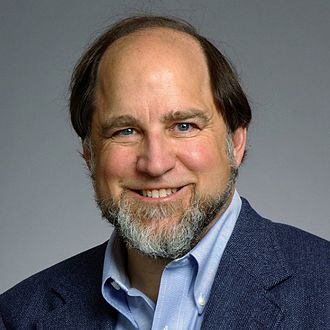
\includegraphics[scale=0.4]{figs/Rivest.jpg}\\
% Ron Rivest 
% \end{column}
% \begin{column}{0.33\textwidth}
% \centering
% 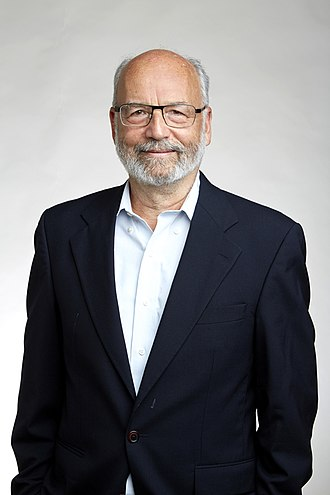
\includegraphics[scale=0.3]{figs/Shamir.jpg}\\
% Adi Shamir
% \end{column}
% \begin{column}{0.33\textwidth}
% \centering
% 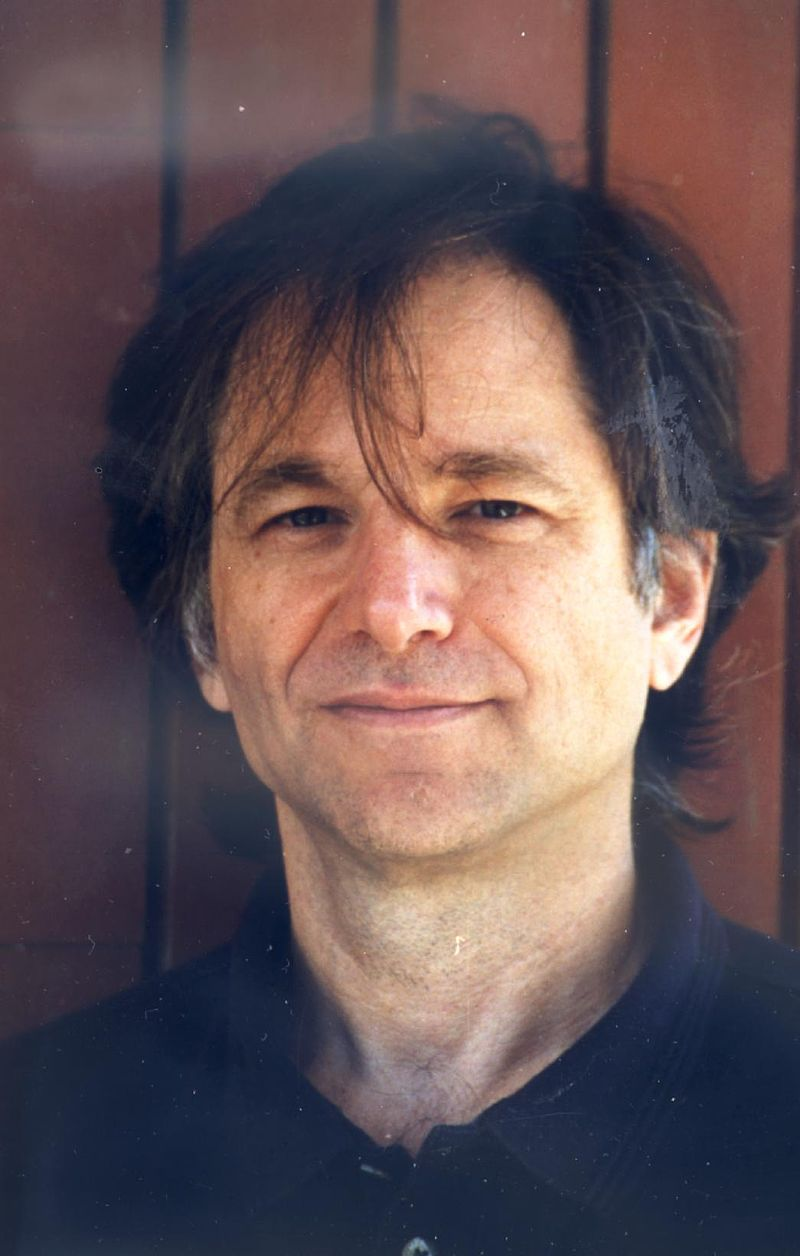
\includegraphics[scale=0.1]{figs/Adleman.jpg}\\
% Leonard Adleman
% \end{column}
% \end{columns}
% \end{frame}


% \begin{frame}{}{}
% O RSA depende de algumas facetas da Teoria dos Números, uma delas é a {\bf aritmética modular}.
% \begin{itemize}
% \pitem Na aritmética modular escolhemos um inteiro positivo $n$ e sempre que chegamos a $n$ imediatamente voltamos a 0.
% \pitem É como aritmética em um relógio, sempre que chega a 12, voltamos para 0. Se você vai dormir as 11 e dorme 8 horas, você acorda as 7. 
% \end{itemize}
% \end{frame}

% \begin{frame}{}{}
% \begin{itemize}
% \pitem É como aritmética com inteiros, mas sempre dividimos por $n$ e tomamos o resto. Por exemplo, em uma aritmética módulo 5 os únicos valores possíveis são 0, 1, 2, 3 e 4.
% \pitem Em módulo 5:
% $$
% 3 + 4 \equiv 2
% $$
% \pitem Pois 7 dividido por 5 tem resto 2. Definimos um operador $\bmod$ para essa operação. de forma que $7 \bmod 5 = 2$
% \end{itemize}
% \end{frame}

% \begin{frame}{}{}
% O operador $\bmod$ tem algumas propriedade interessantes:
% \begin{itemize}
% \pitem  $(a + b) \bmod n = ((a \bmod n) + (b \bmod n)) \bmod n$,
% \pitem  $ab \bmod n = ((a \bmod n)(b \bmod n)) \bmod n$,
% \pitem  $a^b \bmod n = (a \bmod n)^b \bmod n$.
% \end{itemize}
% \end{frame}


% \begin{frame}{}{}
% \begin{itemize}
% \item Na matemática o {\bf inverso multiplicativo} de um número $x$ é um número $y$ tal que $x \cdot y = 1$. 
% \pitem Na aritmética modular temos uma definição parecida.
% O {\bf inverso multiplicativo } de um número $x$ em {\bf modulo $n$} é um inteiro $y$ tal que 
% $$
% x \cdot y \bmod n \equiv 1 \bmod n 
% $$
% \pitem Por exemplo o inverso multiplicativo em módulo 5 de 3 é 2 pois
% $$
% 3 \cdot 2 \bmod 5 = 6 \bmod 5 \equiv 1\bmod 5
% $$
% \end{itemize}
% \end{frame}



% \begin{frame}{}{}
% \begin{itemize}
% \item Note que se $x$ e $n$ tem fatores em comum por exemplo $x = 2$ e $n = 6$ não existe inverso multiplicativo.
% \begin{align*}
% 2 * 1 \bmod 6 &= 2 \bmod 6 \\
% 2 * 2 \bmod 6 &= 4 \bmod 6\\
% 2 * 3 \bmod 6 &= 6 \bmod 6 \equiv 0 \bmod 6\\
% 2 * 4 \bmod 6 &= 8 \bmod 6 \equiv 2 \bmod 6\\
% 2 * 5 \bmod 6 &= 10 \bmod 6 \equiv 4 \bmod 6
% \end{align*}
% \pitem Mas se $x$ e $n$ são primos relativos o inverso multiplicativo existe.
% \end{itemize}
% \end{frame}

% \begin{frame}{}{}
% \ppause
% No {\bf sistema de criptografia de chave pública RSA} um participante cria suas chaves públicas e secreta com o seguinte procedimento:
% \begin{enumerate}
% \pitem Seleciona aleatoriamente dois números primos grandes (de pelo menos 1024 bits) distintos $p$ e $q$.
% \pitem Calcule $n = pq$ (Esse número tem pelo menos 2048 bits ou 618 dígitos decimais.)
% \pitem Calcule $r = (p-1)(q-1)$ que é quase tão grande quando $n$
% \end{enumerate}

% \end{frame}


% \begin{frame}{}{}
% \begin{enumerate}
% \setcounter{enumi}{3}
% \item Seleciona um inteiro ímpar pequeno $e$ tal que $e$ seja {\bf relativamente primo} de $r$, ou seja, o único divisor comum é 1. Qualquer inteiro pequeno serve.
% \pitem Calcule $d$ como o {\it inverso multiplicativo} de $e$, módulo $r$. Isto é $e d \bmod r$ deve ser igual a 1.
% \pitem Divulgue o par $P = (e, n)$ como a chave pública.
% \pitem Mantenha $S = (d, n)$ em segredo como a chave secreta.
% \end{enumerate}
% \end{frame}

% \newcommand{\mmod}{\texttt{mod}\ }
% \begin{frame}{}{}
% \begin{itemize}
% \pitem Para criptografar uma mensagem $M$ fazemos
% $$
% F_P(M) = M^e (\mmod n)
% $$
% \pitem Para transformar um texto cifrado C:
% $$
% F_S(C) = C^d (\mmod n)
% $$
% \end{itemize}
% \end{frame}

% \begin{frame}{Exemplo}{}
% \begin{itemize}
% \pitem Bob sorteia $p = 17$ e $q = 29$ (Na prática sorteia números de no mínimo 1024 bits)
% \pitem Calcula $n = pq = 493$
% \pitem Calcula $r = (p-1)(q-1) = 448$
% \pitem Seleciona $e = 5$ que é um primo relativo de $448$
% \pitem Calcula $d = 269$, já que $5\cdot 269 \bmod r = 1345 \bmod r = 1$
% \pitem Publica a chave $P = (5, 493)$
% \pitem Guarda com carinho a chave $S = (269, 493)$
% \end{itemize}
% \end{frame}


% \begin{frame}{}{}
% Chaves de Bob $P = (5, 493)$ e $S = (269, 493)$
% \begin{itemize}
% \pitem Alice quer enviar a mensagem 327
% \begin{align}
% F_P(327) & = 327^5 \bmod 493 \\\ppause
% & = 3.738.856.210.407 \bmod 493 \\\ppause
% & = 259
% \end{align}
% \end{itemize}
% \end{frame}


% \begin{frame}{}{}
% \begin{itemize}
% \pitem Na verdade Alice não precisa lidar com números astronômicos. (iclusive muito maiores que esse)
% \begin{align}
% 327^5 \bmod 493 \\
% 327^2 \cdot 327^3 \bmod 493 \\
% (327^2 \bmod 493 \cdot 327^3 \bmod 493) \bmod 493 \\
% (106929 \bmod 493 \cdot 327^3 \bmod 493) \bmod 493 \\  
% (441 \cdot 327^3 \bmod 493) \bmod 493 \\  
% (441 \cdot 441 \cdot 327 \bmod 493) \bmod 493 \\  
% 78153 \bmod 493 = 259
% \end{align}
% \end{itemize}
% \end{frame}

% \begin{frame}{}{}
% Chaves de Bob $P = (5, 493)$ e $S = (269, 493)$
% \begin{itemize}
% \item Bob então recebe a mensagem criptografada $C = 259$. E decifra ela:
% $$
% F_S(259) = 259^{269} \bmod 493 =\ppause 327
% $$
% \pitem Que de fato é a mensagem original de Alice!
% \end{itemize}
% \end{frame}


% \begin{frame}{Corretude do RSA}{Mostrando que $F_P$ e $F_S$ são inversas uma da outra}
% \begin{itemize}
% \item Para criptografar um texto $M$ fazemos: $F_P(M) = M^e (\bmod n)$
% \item Para transformar um cifrado C: $F_S(C) = C^d (\bmod n)$
% \end{itemize}
% \ppause
% O sistema RSA de fato é capaz de encriptar e decodificar mensagens 
% \begin{align*}
% F_S(F_P(M)) & = F_S(M^e (\bmod n)) \\
%         & = (M^e (\bmod n))^d (\bmod n)\\
%         & = M^{ed} (\bmod n)
% \end{align*}
% \end{frame}


% \begin{frame}{}{}
% \begin{itemize}
% \pitem Queremos mostrar então que $$M^{ed} (\bmod n) = M \bmod n$$ e como $M < n$ então $$M \bmod n = M$$
% \pitem Começaremos mostrando que $$M^{ed} (\bmod p) = M (\bmod p)$$
% \end{itemize}
% \end{frame}



% \begin{frame}{}{}
% \begin{itemize}
% \pitem Lembrando que $r = (p-1)(q-1)$,
% \pitem e que $e$ é um primo relativo de $r$,
% \pitem e que $d$ é um inverso multiplicativo de e em aritmética módulo $r$, o que equivale a dizer que existe um inteiro $h$ tal que:
% $$
% ed = 1 + h(p-1)(q-1)
% $$
% \end{itemize}
% \end{frame}

% \begin{frame}{}{}
% \begin{itemize}
% \pitem Seja $\mathbb{Z}_p = \{0,1,\ldots, n-1\}$
% \pitem Seja $\mathbb{Z}_p^*$ o conjunto dos elementos de $\mathbb{Z}_p$ que são primos relativos de $p$. Ou seja, se $a \in \mathbb{Z}_p^*$ então $mdc(p, a) = 1$. \ppause
% \end{itemize}
% \begin{block}{Pequeno teorema de Fermat}{}
% Seja $p$ um número primo e $a \in \mathbb{Z}_p^*$, então 
% $$
% a^{p - 1} \equiv 1 (\bmod p)
% $$
% \end{block}

% \end{frame}


% \begin{frame}{}{}
% {\bf Prova:}

% Considere a sequência $L = (a, 2a, 3a, \ldots, (p-1) a)$ de $(p-1)$ múltiplos de a.
% \begin{itemize}
% \pitem Nenhum é múltiplo de $p$ já que $a$ e $p$ são primos relativos. E para todo $ka \in L$, $k \leq (p-1)$.
% \pitem Em $L$ não tem 2 elementos congruentes em módulo $p$. 

% \end{itemize}
% \end{frame}


% \begin{frame}{}{}
% \begin{itemize}
% \pitem Suponha por absurdo que exitem $k_1, k_2 \in \{1, 2, \ldots, p-1\}$
% com $k_1 \neq k_2$ tal que
% \begin{align}
% a k_1 \bmod p &\equiv a k_2 \bmod p 
% \end{align}\ppause
% Seja $a'$ o inverso multiplicativo de $a$.
% \begin{align}
% a' a k_1 \bmod p &\equiv a' a k_2 \bmod p \\
% k_1 \bmod p &\equiv k_2 \bmod p 
% \end{align}\ppause
% Como $k_1$ e $k_2$ são menores que $p$
% \begin{align}
% k_1 = k_2 \ppause (ABSURDO)
% \end{align}
% \end{itemize}
% \end{frame}

% \begin{frame}{}{}
% {\bf Prova:}

% Considere a sequência $L = (a, 2a, 3a, \ldots, (p-1) a)$ de $(p-1)$ múltiplos de a.
% \begin{itemize}
% \item Nenhum é múltiplo de $p$ já que $a$ e $p$ são primos relativos. E para todo $ka \in L$, $k \leq (p-1)$.
% \item Em $L$ não tem 2 elementos congruentes em módulo $p$. 
% \pitem Cada $l \in L$ então é congruente a $\{1, 2, \ldots, p-1\}$
% \begin{align}
% a \cdot 2a \ldots (p-1)a &\equiv 1 \cdot 2 \ldots (p-1) (\bmod p)\\
% a^{p-1}.(p-1)! &\equiv  (p-1)! (\bmod p)\\
% a^{p-1} &\equiv  1 (\bmod p)
% \end{align}
% \end{itemize}
% \end{frame}



% \begin{frame}{}{}
% \begin{align*}
% &M^{ed} (\bmod p) \\\ppause
% &= (M \bmod p)^{ed} \bmod p\\\ppause
% &= (M \bmod p)^{1 + h(p-1)(q-1)} \bmod p\\\ppause
% &= (M \bmod p)\cdot (M \bmod p)^{h(p-1)(q-1)} \bmod p\\\ppause
% &= (M \bmod p)\cdot ((M \bmod p)^{(p-1)})^{h(q-1)} \bmod p\\\ppause
% &= (M \bmod p)\cdot ((M \bmod p)^{(p-1)} \bmod p)^{h(q-1)} \bmod p\\\ppause
% &= (M \bmod p)\cdot (1)^{h(q-1)} \bmod p\\\ppause
% &= (M \bmod p)
% \end{align*}
% \end{frame}





% \begin{frame}{}{}
% \begin{itemize}
% \item Analogamente $M^{ed} (\bmod q) = (M \bmod q)$.
% \pitem Além disso se 
% $$x \bmod p = y \bmod p$$
% e 
% $$x \bmod q = y \bmod q$$
% então 
% $$x \bmod pq = y \bmod pq$$
% \end{itemize}
% \end{frame}







% \begin{frame}{}{}
% \begin{itemize}
% \pitem Como $M^{ed} (\bmod p) = M \bmod p$,
% \pitem e $M^{ed}  \bmod q = M \bmod q$
% \pitem então $$M^{ed} (\bmod pq) = M \bmod pq$$
% \pitem Como $pq = n$
% \item então $$M^{ed} (\bmod n) = M \bmod n$$
% \item e portanto a chave secreta de Bob decifra $C$
% \end{itemize}
% \end{frame}



% \begin{frame}{}{}
% \begin{itemize}
% \pitem Além disso, talvez você tenha reparado que se Bob cifrar um texto comum com a sua chave secreta $S = (d, n)$:
% $$
% F_S(M) = M^{d} (\bmod n)
% $$
% \pitem Alice pode decifra-la com a chave pública. 
% $$
% F_P(M^{d} (\bmod n)) = M^{de} (\bmod n) =  M^{ed} (\bmod n) = M
% $$
% \pitem Isso não tem muita utilidade se o objetivo era esconder $M$ já que todo mundo conhece $P$. 
% \end{itemize}
% \end{frame}


% \begin{frame}{}{}
% \begin{itemize}
% \pitem Entretanto serve para Bob provar que foi ele quem escreveu $M$. Já que ninguém mais conseguiria cifrar $M$ dessa forma.
% \pitem Se Bob então enviar $M$ e $F_S(M)$, Alice e quem mais quiser terá certeza que foi Bob que enviou a mensagem.
% \pitem Além disso se Bob enviar $M$ e $F_S(M)$, Alice terá certeza que a mensagem $M$ não foi corrompida por exemplo.
% \end{itemize}
% \end{frame}

% \begin{frame}{}{}
% \begin{itemize}
% \pitem Note que Alice pode gerar as suas próprias chaves e Bob também poderá enviar mensagens cifradas que só ela poderá ler.
% \pitem Além disso se toda a codificação e decodificação usando aritmética  modular for pesado para a quantidade de informações que Alice e Bob querem trocar. Eles podem usar o RSA para trocar chaves simétricas que sejam mais rápidas de calcular.
% \end{itemize}
% \end{frame}

%
%\begin{frame}{}{}
%\begin{itemize}
%\pitem 
%\end{itemize}
%\end{frame}
%
%
%\begin{frame}{}{}
%     \begin{columns}[T] % contents are top vertically aligned
%     \begin{column}{0.6\textwidth} 
%     \end{column}
%     \begin{column}{0.4\textwidth} % alternative top-align that's better for graphics
%     \end{column}
%     \end{columns}
%\end{frame}
%
%
%\begin{frame}{}{}
%\begin{itemize}
%\pitem 
%\end{itemize}
%\end{frame}
%
%\begin{frame}{}{}
%\begin{itemize}
%\pitem 
%\end{itemize}
%\end{frame}
%
%\begin{frame}{}{}
%\begin{itemize}
%\pitem 
%\end{itemize}
%\end{frame}

%\input{mod26_BackTracking_Limitantes_BnB}
%\input{aula_PL}
%\input{aula_PLI} % as formulações dessa aula são feitas na lousa
%\input{aula_PLI_CP}
\end{document}
